\usepackage{graphicx}

\section{Fonctionnement}

\subsection{Organisation}
\paragarphe{}Notre équipe est composée de trois membres à la charge du projet : Karabouali Makoura
, Phetramphand Antoine et Tangara Ramatoulaye.
Pour mieux appréhender le projet, nous avons entamé des recherches et approfondir les non acquis
et mettre le problème en oeuvre techniquement en utilisant le processus «modèle en cascade»
\vspace{10mm}
\paragarphe{}Chaque semaine, nous nous sommes réunis pour réfléchir à l'avancement de nos différents travaux et voir les solutions possibles en cas d'erreur.Et pour mieux travailler en parallèle, nous avons utilisé les messages électroniques afin de s'informer sur l'avancemeent de nos travaux respectifs pour permettre de mieux fixer la prochaine mise en commun.

\vspace{10mm}
\paragarphe{}Tout d'abord, nous avons commencé par le développement du mode console, puis du mode graphique car celui-ci utilise une partie du code du mode console.
Pour chaque avancement nous avons établi des tests afin d'être certain du bon fonctionnement avant de passer à autre chose.
 
\vspace{10mm}


\subsection{Réalisation}
\label{sec:impl}
\paragraph{} Pour pouvoir bien mener le projet 
nous avons suivi les étapes suivantes :

\begin{itemize} 
   \item{1ème Etape : Recherches}
   \paragraphe{}Nous avons effectué des recherches sur internet ainsi que des recherches bibliographique sur notre sujet afin d'approfondir et mieux résoudre le problème.
	
	
   \item{2ème Etape : Répartition des tâches}
	\paragraphe{}Le sujet étant libre, nous devions nous fixer notre propre cahier des charges. Nous avons décidé de fonctionner avec 				plusieurs versions. Pour chaque nouvelle version, nous nous réunissions pour conceptualiser un nouveau problème et une nouvelle solution (nouveau cahier des charge), puis après avoir défini le diagramme UML de notre projet, nous nous répartissions les tâches pour effectuer chacun une partie du travail. Enfin, nous nous réunissions pour mettre en commun, effectuer une batterie de test et corriger les éventuelles erreurs.
\paragraphe{}Cependant, chacun avait des tâches prioritaires à accomplir.
\begin{table}[h!]
\centering
\begin{tabular} {|p{2.5cm}|p{5.5cm}|p{2cm}|}
\hline
Tâches & Personne\\
\hline
mode graphique & Antoine\\
\hline
mode console & Ramatoulaye\\
\hline
documentation & Makoura \\
\hline
\end{tabular}
\caption{Répartition des tâches}
\label{tab:document}
\end{table}

\item{3ème étape : développement des classes}
\paragraph{}Pour développer nos classes, nous nous sommes tout d'abord basés sur le diagramme UML suivant :

\begin{center}
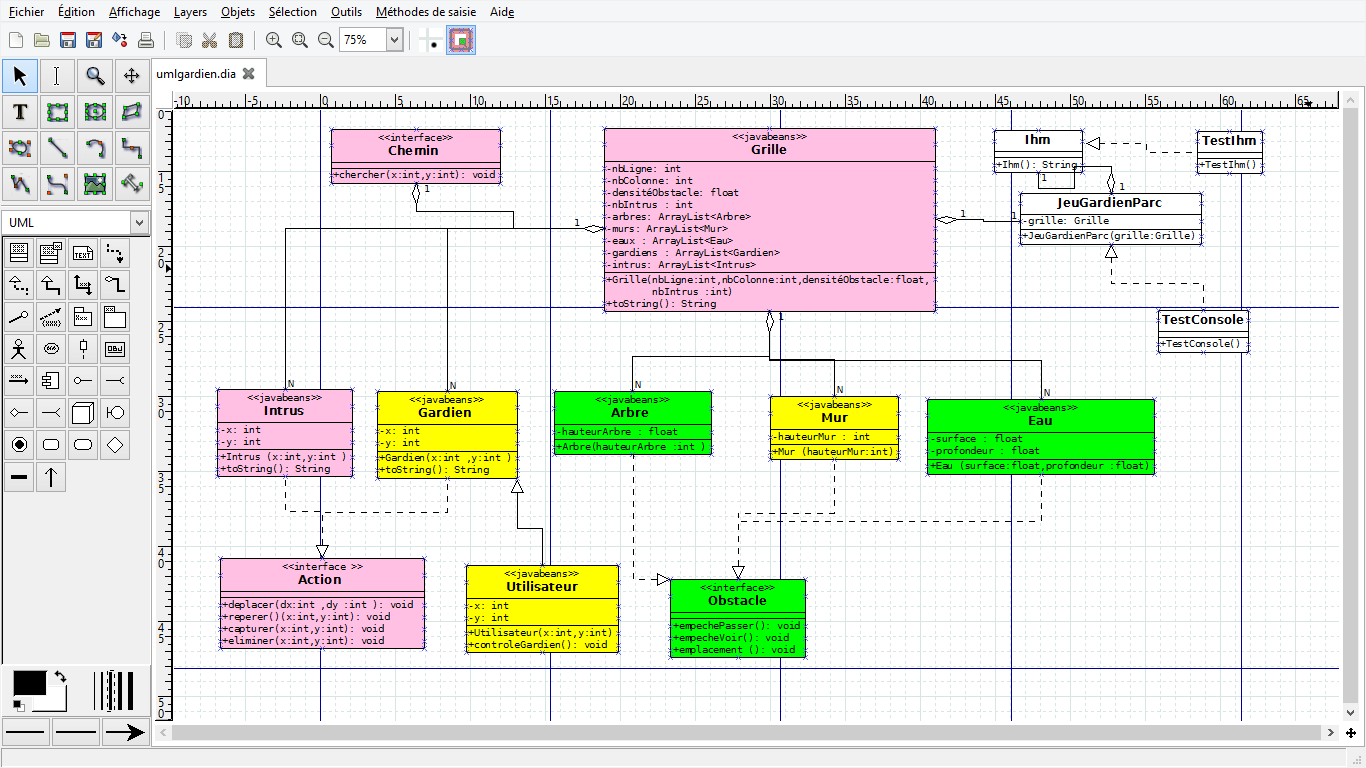
\includegraphics[height=200, width=400]{images/uml_debut.png}
\end{center}
\paragraphe{}Puis par la suite, nous nous sommes rendus compte que la version conçue n'était pas celle qui nous fallait car elle ne permettait pas à l'utilisateur de choisir ces propres dimensions (taille de la grille), ni de placer lui-même les éléments ou encore de choisir le nombre d'éléments qu'il souhaite mettre ne place. Nous en sommes venus alors après élaborations de plusieurs versions à la version finale dont le digramme UML est le suivant : 

\begin{center}
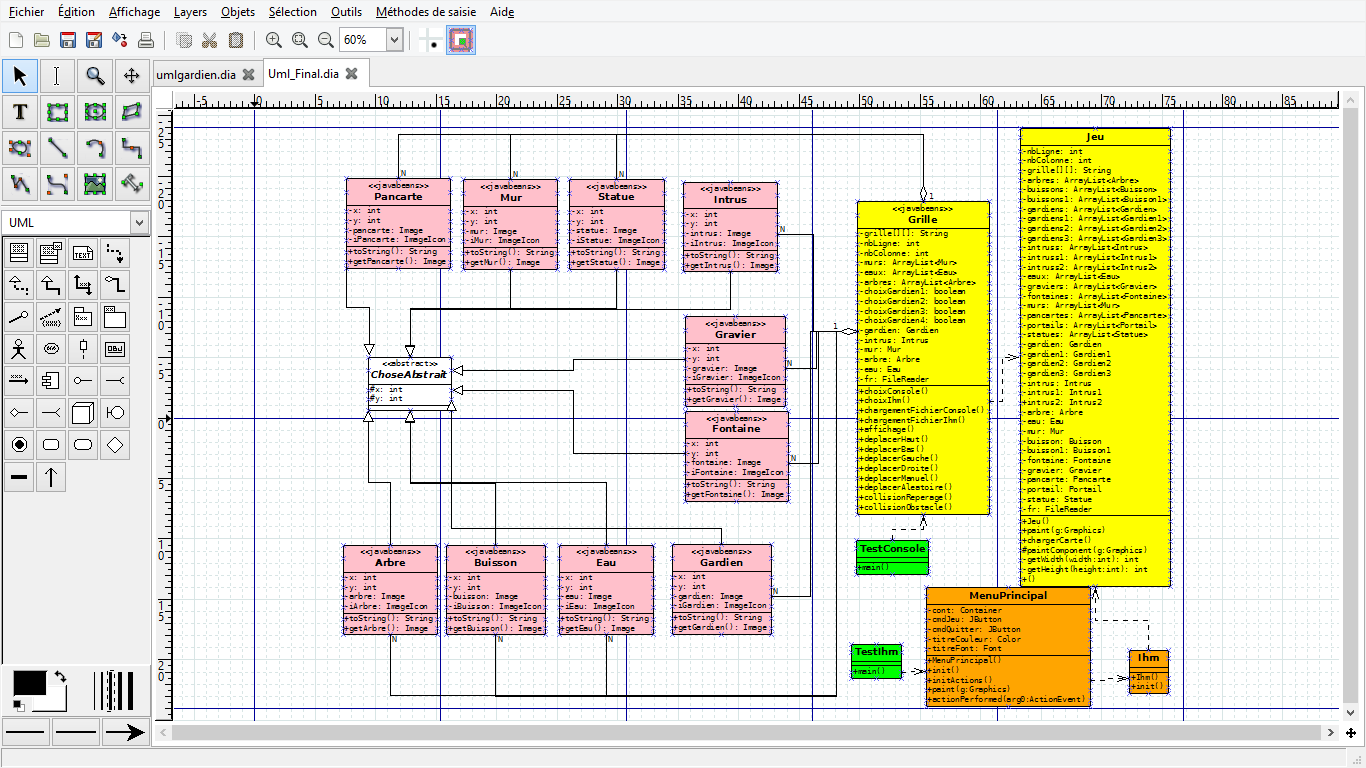
\includegraphics[height=200, width=400]{images/uml_final.png}
\end{center}
\paragraphe{}Cette version donne plus de liberté qu'auparavant.
\end{itemize}
